\documentclass[acmtog]{acmart}
\usepackage{graphicx}
\usepackage{subfigure}
\usepackage{natbib}
\usepackage{listings}
\usepackage{bm}
\usepackage{amsmath}

\definecolor{blve}{rgb}{0.3372549 , 0.61176471, 0.83921569}
\definecolor{gr33n}{rgb}{0.29019608, 0.7372549, 0.64705882}
\makeatletter
\lst@InstallKeywords k{class}{classstyle}\slshape{classstyle}{}ld
\makeatother
\lstset{language=C++,
	basicstyle=\ttfamily,
	keywordstyle=\color{blve}\ttfamily,
	stringstyle=\color{red}\ttfamily,
	commentstyle=\color{magenta}\ttfamily,
	morecomment=[l][\color{magenta}]{\#},
	classstyle = \bfseries\color{gr33n}, 
	tabsize=2
}
\lstset{basicstyle=\ttfamily}

% Title portion
\title{Assignment 3:\\ {Ray Tracing with Direct Lighting}} 

\author{Name:\quad 张厶元  \\ student number:\ 2019533240
\\email:\quad zhangsy3@shanghaitech.edu.cn}

% Document starts
\begin{document}
\maketitle

\vspace*{2 ex}

\section{Introduction}
\begin{itemize}
\item a pin-hole camera model, which is able to shoot a set of optical rays. And there should be at least one ray per pixel.
\item the algorithm for the ray-triangle intersection (without the acceleration structure).
\item the algorithm for the ray-cube intersection based on the ray-triangle intersection (without the acceleration structure).
\item anti-aliasing for ray-tracing by using super-sampling with the rotated grid.
\end{itemize}
\section{Implementation Details}
\subsection{Pin-hole Camera Model and Ray Generate}
\begin{figure}[h]
	\centering
	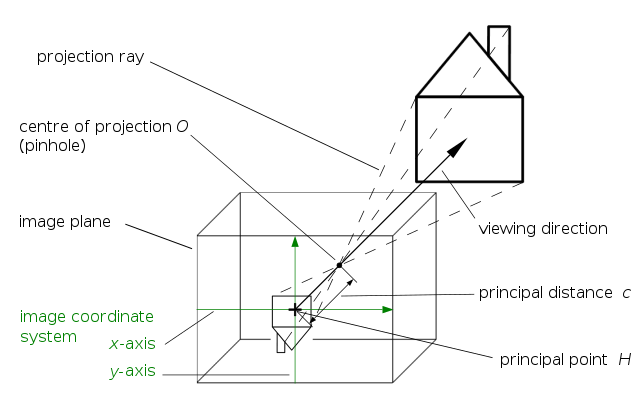
\includegraphics[height = 4.5cm]{Pinhole_camera_model.png}
	\caption{Pinhole Camera Model}
\end{figure}
\begin{equation}
\begin{split}
	Forward &= Position - LookAt \\
	Right &= RefUp \times Forward \\
	Up &= Forward \times Right \\
\end{split}
\end{equation}

And for the ray generation, we just need to calculate the ray direction and the ray origin position, which is from a pixel on the camera panel to the position and go through the pinhole, and we can use a transformation
\begin{figure}[h]
	\centering
	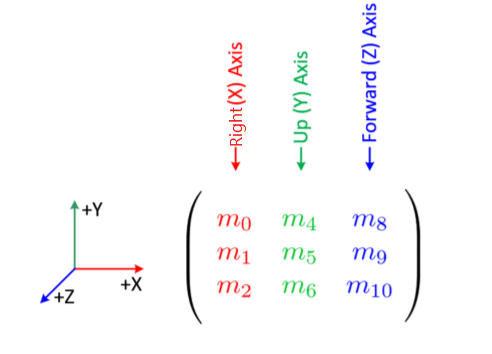
\includegraphics[height = 3cm]{transformation.png}
	\caption{transformation}
\end{figure}

\begin{equation}
\begin{split}
	CameraPosition &= (px,py,-f) \\
	RealWorldPosition &= trans \cdot CameraPosition + RealWorldCamPos \\
	RealWorldRayDirection &= trans \cdot CameraPosition \\
\end{split}
\end{equation}

\subsection{Ray-Triangle Intersection}
Then we follow the Möller-Trumbore algorithm to test whether the ray hits the triangle as follows:
\begin{lstlisting}[language=C++]
bool RayIntersectsTriangle(Vector3D rayOrigin,
Vector3D rayVector,
Triangle* inTriangle,
Vector3D& outIntersectionPoint)
	{
	const float EPSILON = 0.0000001;
	Vector3D vertex0 = inTriangle->vertex0;
	Vector3D vertex1 = inTriangle->vertex1;
	Vector3D vertex2 = inTriangle->vertex2;
	Vector3D edge1, edge2, h, s, q;
	float a,f,u,v;
	edge1 = vertex1 - vertex0;
	edge2 = vertex2 - vertex0;
	h = rayVector.crossProduct(edge2);
	a = edge1.dotProduct(h);
	if (a > -EPSILON && a < EPSILON)
	return false;
    // This ray is parallel to this triangle.
	f = 1.0/a;
	s = rayOrigin - vertex0;
	u = f * s.dotProduct(h);
	if (u < 0.0 || u > 1.0)
	return false;
	q = s.crossProduct(edge1);
	v = f * rayVector.dotProduct(q);
	if (v < 0.0 || u + v > 1.0)
	return false;
	// At this stage we can compute t to find out
    // where the intersection point is on the line.
	float t = f * edge2.dotProduct(q);
	if (t > EPSILON) // ray intersection
		{
		outIntersectionPoint = rayOrigin +
                               rayVector * t;
		return true;
	}
	else
    // This means that there is a line intersection
    // but not a ray intersection.
	return false;
}
\end{lstlisting}
\subsection{Area light}
 Seeing that we are rendering the scene with a panel of light, not a spot light, so we should sample the light source with a uniform distribution and distribute the lumen.
So each sample is only one n\textsuperscript{th} of the original light source.
\subsection{integrator}
\subsubsection{radiance}
Seeing that we don't care the reflection for now, we just have two conditions: the ray hit the light, or the ray hit the object.\\
For case one, we just set the color to the light's color as we can see the light color directly from the camera. \\
For case two, we need to calculate the color of the object by using the Phong model.
As same as the muti-light model in the project one, we can calculate the BRDF of each light source and sum all the BRDFs. Moreover we should test whether the ray can touch the light without be shadowed by other objects.
\begin{equation}
	L_o(p,\omega_o) = \sum_{L_i}brdf(p)\cdot L_i \cos{\theta_i} \Delta A
\end{equation}
and just use the phong model to calculate the diffusion and specular
\subsubsection{rendering}
Trace the ray from the camera to the world pixel by pixel.
\begin{itemize}
	\item 1) generate ray.
	\item 2) insert into the scene.
	\item 3) get the radiance.
	\item 4) set pixel.
\end{itemize}


\subsection{Anti-Aliasing}
\begin{figure}[h]
	\centering
	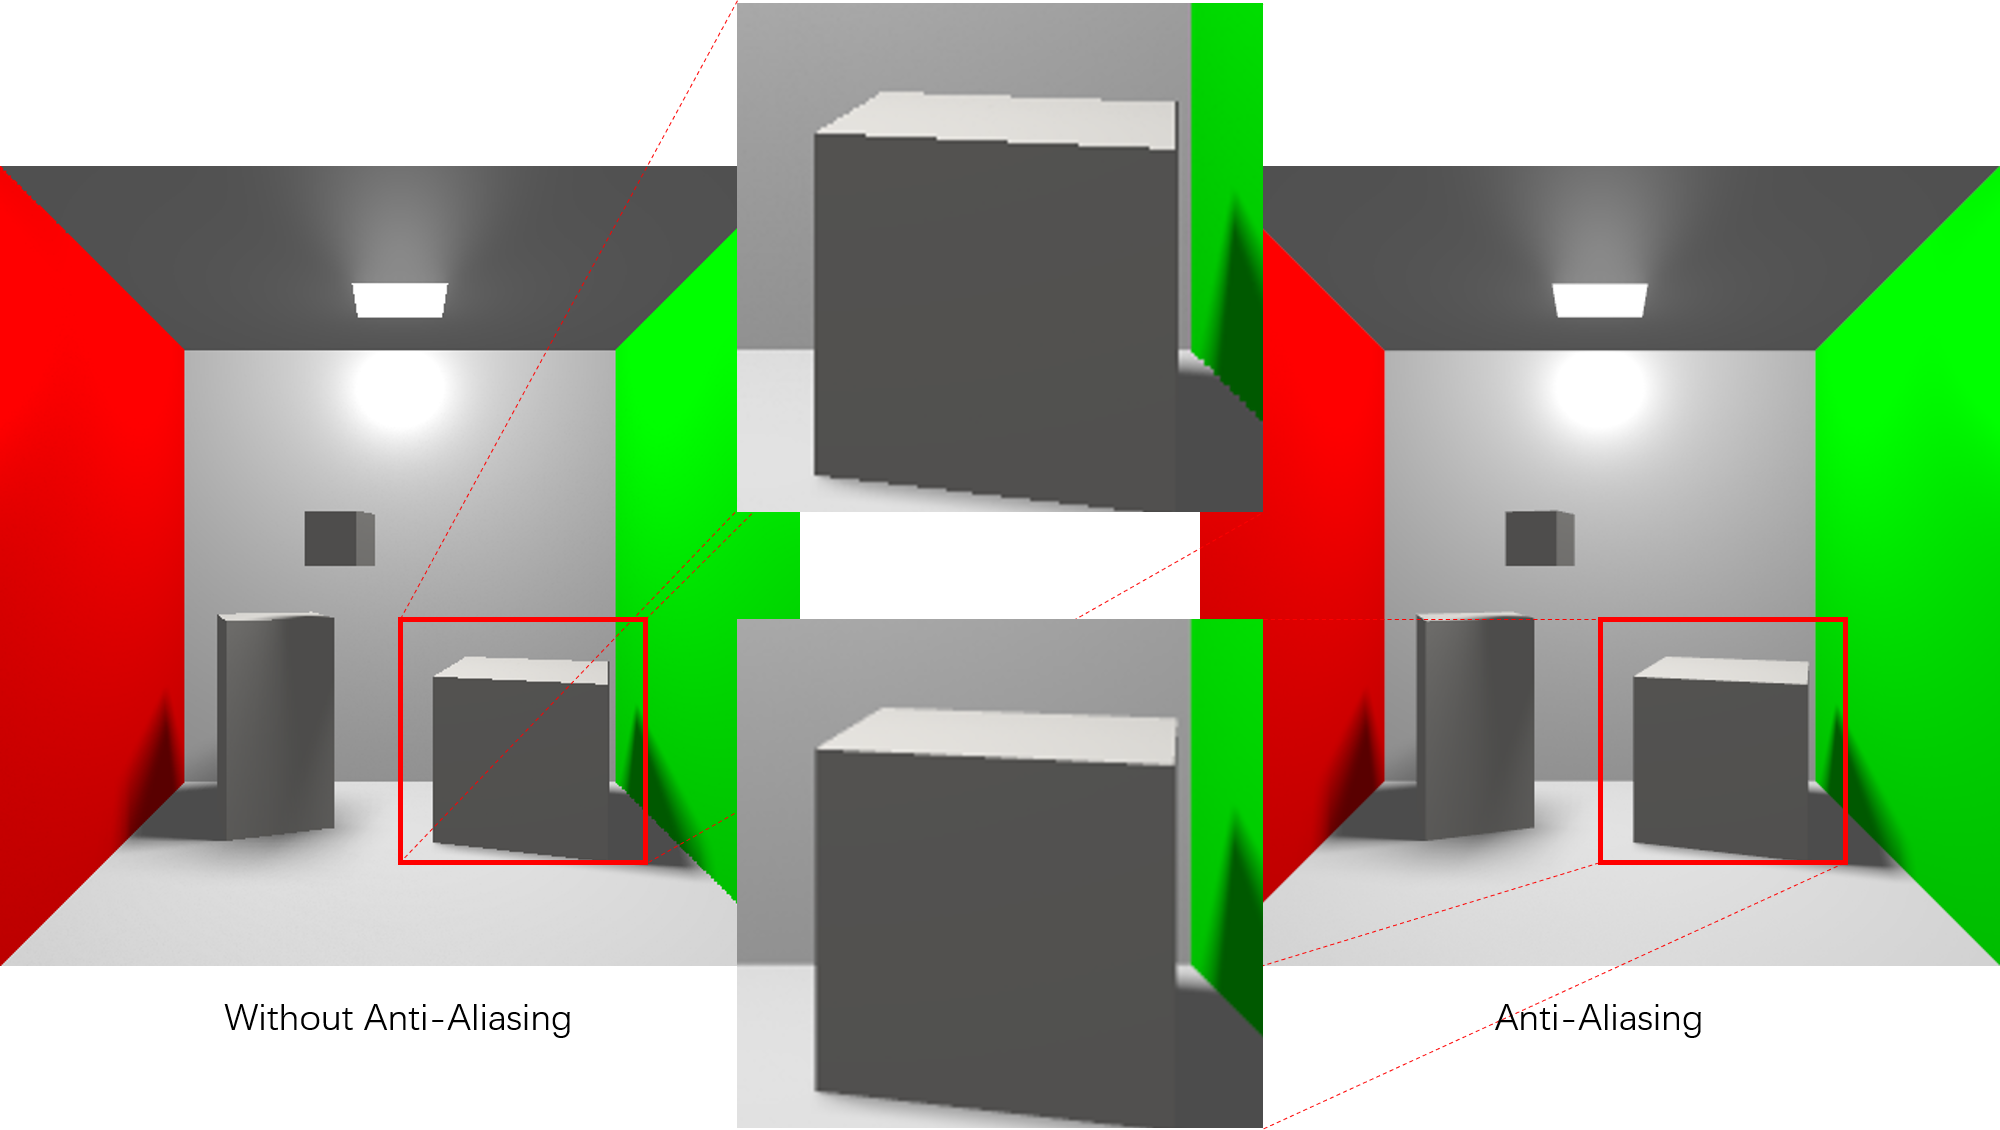
\includegraphics[height = 5cm]{anti-aliasing.png}
	\caption{comparison of the output of anti-alising and without anti-alising}
\end{figure}
By using up sampling and with rotated grid pattern, we can reduce the aliasing effect of the image.

\begin{lstlisting}[language=C++]
for (int i = 0; i < num_sample; i++) {
	for (int j = 0; j < num_sample; j++) {
		vec2f beam_origin(
		pixel_pos.x() + pixel_size.x() * (i + 0.5f) / num_sample,
		pixel_pos.y() + pixel_size.y() * (j + 0.5f) / num_sample);

		vec2f offset = beam_origin - center_pos;
		beam_origin = rotate_matrix * offset + center_pos;
		...
		generateray();
		insert();
		getradiance();
		setpixel();
	}
}
\end{lstlisting}
\section{Results}
\begin{figure}[h]
	\centering
	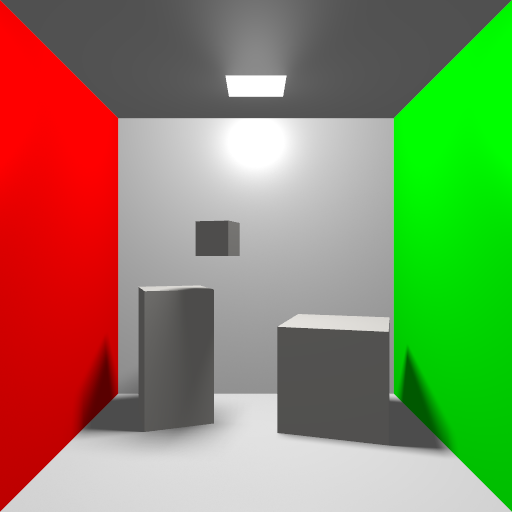
\includegraphics[height = 7.5cm]{output1.png}
	\caption{case 1}
\end{figure}
\begin{figure}[h]
	\centering
	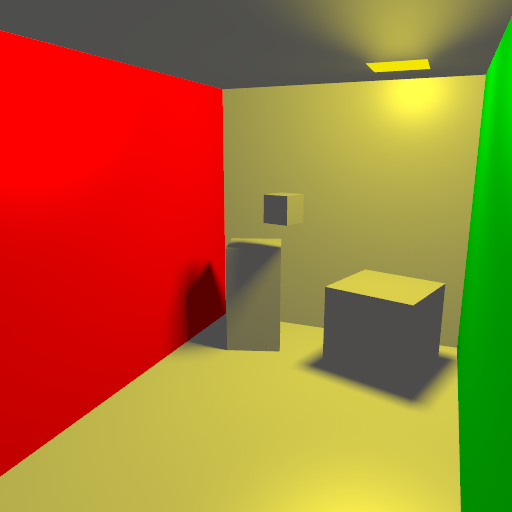
\includegraphics[height = 7.5cm]{output2.png}
	\caption{case 2}
\end{figure}
\begin{figure}[h]
	\centering
	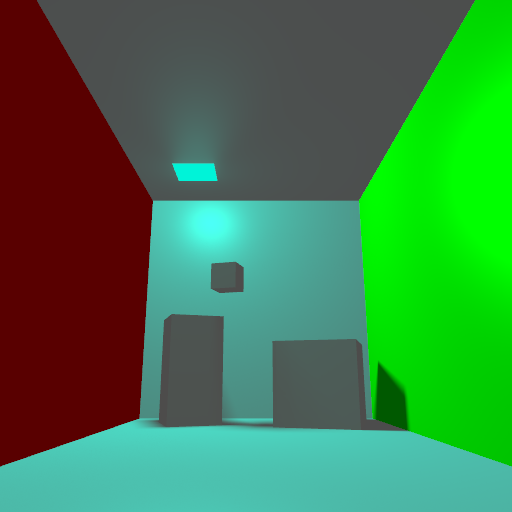
\includegraphics[height = 7.5cm]{output3.png}
	\caption{case 3}
\end{figure}
\\
\end{document}
